% --------------------------------------------------------------
% This is all preamble stuff that you don't have to worry about.
% Head down to where it says "Start here"
% --------------------------------------------------------------
 
\documentclass[12pt]{article}
 
\usepackage[margin=1in]{geometry} 
\usepackage{amsmath,amsthm,amssymb}
\usepackage{xcolor}
\usepackage{listings}
\usepackage{graphicx}
\usepackage{hyperref}
\usepackage{listings}
\usepackage{stackengine}
\usepackage{array}
\usepackage{booktabs}
\usepackage{siunitx}
\graphicspath{{/home/arpit/Desktop/iitd/sem_7/COL334/projects/Getting-To-Know-Network-Traffic/img}}

\newcommand{\N}{\mathbb{N}}
\newcommand{\Z}{\mathbb{Z}}
 
\newenvironment{theorem}[2][Theorem]{\begin{trivlist}
\item[\hskip \labelsep {\bfseries #1}\hskip \labelsep {\bfseries #2.}]}{\end{trivlist}}
\newenvironment{lemma}[2][Lemma]{\begin{trivlist}
\item[\hskip \labelsep {\bfseries #1}\hskip \labelsep {\bfseries #2.}]}{\end{trivlist}}
\newenvironment{exercise}[2][Exercise]{\begin{trivlist}
\item[\hskip \labelsep {\bfseries #1}\hskip \labelsep {\bfseries #2.}]}{\end{trivlist}}
\newenvironment{problem}[2][Problem]{\begin{trivlist}
\item[\hskip \labelsep {\bfseries #1}\hskip \labelsep {\bfseries #2.}]}{\end{trivlist}}
\newenvironment{question}[2][Question]{\begin{trivlist}
\item[\hskip \labelsep {\bfseries #1}\hskip \labelsep {\bfseries #2.}]}{\end{trivlist}}
\newenvironment{corollary}[2][Corollary]{\begin{trivlist}
\item[\hskip \labelsep {\bfseries #1}\hskip \labelsep {\bfseries #2.}]}{\end{trivlist}}

\newenvironment{solution}{\begin{proof}[Solution]}{\end{proof}}
\definecolor{codegreen}{rgb}{0,0.6,0}
\definecolor{codegray}{rgb}{0.5,0.5,0.5}
\definecolor{codepurple}{rgb}{0.58,0,0.82}
\definecolor{backcolour}{rgb}{0.95,0.95,0.92}

\lstdefinestyle{mystyle}{
    backgroundcolor=\color{backcolour},   
    commentstyle=\color{codegreen},
    keywordstyle=\color{magenta},
    numberstyle=\tiny\color{codegray},
    stringstyle=\color{codepurple},
    basicstyle=\ttfamily\footnotesize,
    breakatwhitespace=false,         
    breaklines=true,                 
    captionpos=b,                    
    keepspaces=true,                 
    numbers=left,                    
    numbersep=5pt,                  
    showspaces=false,                
    showstringspaces=false,
    showtabs=false,                  
    tabsize=2
}
\lstset{style=mystyle}
\begin{document}
 
% --------------------------------------------------------------
%                         Start here
% --------------------------------------------------------------
 
\title{\textbf{Assignment 3: An Introduction to the World of SDN}}
\author{Arpit Prasad and Akshat Bhasin\\ 2022EE11837 and 2022EE31996 \\
\textbf{COL334: Computer Network}}

\maketitle

\section{Part 1: Hub Controller and Learning Switch}

\subsection{pingall Test}

The following are the rules installed in the switches after running \texttt{pingall}:

\begin{enumerate}
    \item \textbf{Hub Controller:}
    \begin{verbatim}
*** s1 ------------------------------------------------------------------------
cookie=0x0, duration=154.396s, table=0, n_packets=83, n_bytes=7966, priority=0 
 actions=CONTROLLER:65535
*** s2 ------------------------------------------------------------------------
cookie=0x0, duration=154.407s, table=0, n_packets=83, n_bytes=7966, priority=0 
 actions=CONTROLLER:65535
    \end{verbatim}

    \item \textbf{Learning Switch Controller:}
    \begin{verbatim}
*** s1 ------------------------------------------------------------------------
cookie=0x0, duration=6.527s, table=0, n_packets=1, n_bytes=98, priority=1,in_port="s1-eth1",dl_src=00:00:00:00:00:01,dl_dst=00:00:00:00:00:02 actions=output:"s1-eth2"
cookie=0x0, duration=6.523s, table=0, n_packets=1, n_bytes=98, priority=1,in_port="s1-eth2",dl_src=00:00:00:00:00:02,dl_dst=00:00:00:00:00:01 actions=output:"s1-eth1"
cookie=0x0, duration=6.514s, table=0, n_packets=1, n_bytes=98, priority=1,in_port="s1-eth1",dl_src=00:00:00:00:00:01,dl_dst=00:00:00:00:00:03 actions=output:"s1-eth3"
cookie=0x0, duration=6.503s, table=0, n_packets=1, n_bytes=98, priority=1,in_port="s1-eth3",dl_src=00:00:00:00:00:03,dl_dst=00:00:00:00:00:01 actions=output:"s1-eth1"
cookie=0x0, duration=6.496s, table=0, n_packets=1, n_bytes=98, priority=1,in_port="s1-eth1",dl_src=00:00:00:00:00:01,dl_dst=00:00:00:00:00:04 actions=output:"s1-eth3"
cookie=0x0, duration=6.488s, table=0, n_packets=1, n_bytes=98, priority=1,in_port="s1-eth3",dl_src=00:00:00:00:00:04,dl_dst=00:00:00:00:00:01 actions=output:"s1-eth1"
cookie=0x0, duration=6.476s, table=0, n_packets=1, n_bytes=98, priority=1,in_port="s1-eth2",dl_src=00:00:00:00:00:02,dl_dst=00:00:00:00:00:03 actions=output:"s1-eth3"
cookie=0x0, duration=6.468s, table=0, n_packets=1, n_bytes=98, priority=1,in_port="s1-eth3",dl_src=00:00:00:00:00:03,dl_dst=00:00:00:00:00:02 actions=output:"s1-eth2"
cookie=0x0, duration=6.462s, table=0, n_packets=1, n_bytes=98, priority=1,in_port="s1-eth2",dl_src=00:00:00:00:00:02,dl_dst=00:00:00:00:00:04 actions=output:"s1-eth3"
cookie=0x0, duration=6.456s, table=0, n_packets=1, n_bytes=98, priority=1,in_port="s1-eth3",dl_src=00:00:00:00:00:04,dl_dst=00:00:00:00:00:02 actions=output:"s1-eth2"
cookie=0xx, duration=14.521s, table=0, n_packets=53, n_bytes=5458, priority=0 actions=CONTROLLER:65535
*** s2 ------------------------------------------------------------------------
cookie=0x0, duration=6.522s, table=0, n_packets=1, n_bytes=98, priority=1,in_port="s2-eth3",dl_src=00:00:00:00:00:01,dl_dst=00:00:00:00:00:03 actions=output:"s2-eth1"
cookie=0x0, duration=6.518s, table=0, n_packets=1, n_bytes=98, priority=1,in_port="s2-eth1",dl_src=00:00:00:00:00:03,dl_dst=00:00:00:00:00:01 actions=output:"s2-eth3"
...
cookie=0x0, duration=14.532s, table=0, n_packets=54, n_bytes=5548, priority=0 actions=CONTROLLER:65535
    \end{verbatim}
\end{enumerate}

The following are the observations of the above results:

\begin{enumerate}
    \item \textbf{Hub Controller Observations:}
        \begin{itemize}
            \item Only a single, low-priority "table-miss" rule is present on each switch.
            \item This rule's action is \texttt{actions=CONTROLLER}, which forces every single packet that the switch does not have a rule for to be sent to the controller.
            \item Since no other rules are ever installed, this means all packets (ARP, ping requests, ping replies) are sent to the controller for a forwarding decision, making the switch effectively "dumb."
        \end{itemize}
    \item \textbf{Learning Switch Observations:}
        \begin{itemize}
            \item Multiple specific, high-priority flow rules are installed on the switches.
            \item Each rule matches on a source/destination MAC address pair and an input port.
            \item This indicates that once the first packet of a conversation is seen, the controller proactively installs a rule on the switch, allowing all subsequent packets of that same conversation to be forwarded directly by the switch hardware at line rate.
            \item The low-priority table-miss rule is still present but handles far fewer packets, as it is only used for the first packet of a new, unknown flow.
        \end{itemize}
\end{enumerate}


\subsection{Throughput Test}

The following are the Throughput of when the following controllers are used:
\begin{enumerate}
    \item Hub Controller: 20.3 Mbits/sec
    \item Learning Switch: 29.1 Gbits/sec
\end{enumerate}

Inferences:
\begin{enumerate}
    \item \textbf{Hub Controller Inference:} The throughput is very low because every data packet in the \texttt{iperf} stream must make a slow, high-latency round trip from the switch to the controller for a forwarding decision. The controller itself becomes the performance bottleneck.
    \item \textbf{Learning Switch Inference:} The throughput is extremely high because the controller only processes the first packet of the flow. It then installs a rule on the switch, allowing all subsequent data packets to be forwarded at the switch's hardware speed (line rate), completely bypassing the controller bottleneck.
\end{enumerate}


\section{Part 2: Layer2-like Shortest Path Routing}

The following are the Testing and Measurements Performed:

\noindent iperf with two parallel TCP Connections:
\begin{enumerate}
    \item \textbf{ECMP Off:}
    \begin{enumerate}
        \item Throughput: 9.50 Mbits/sec
        \item Flow Rules:
        \begin{verbatim}
*** s1 ------------------------------------------------------------------------
cookie=0x0, duration=72.327s, table=0, n_packets=130, n_bytes=7800, 
 priority=65535,dl_dst=01:80:c2:00:00:0e,dl_type=0x88cc actions=CONTROLLER:65535
cookie=0x0, duration=72.338s, table=0, n_packets=42449, n_bytes=4569148, 
 idle_timeout=10, priority=0 actions=CONTROLLER:65535
... (Similar rules on s2-s6) ...
        \end{verbatim}
    \end{enumerate}
    \item \textbf{ECMP On:}
    \begin{enumerate}
        \item Throughput: 19.2 Mbits/sec or 9 Mbits/sec
        \item Flow Rules:
        \begin{verbatim}
*** s1 ------------------------------------------------------------------------
cookie=0x0, duration=20.693s, table=0, n_packets=2123, n_bytes=12329874, 
 idle_timeout=10, priority=20,tcp,nw_src=10.0.0.1,nw_dst=10.0.0.2,tp_src=51634,tp_dst=5001 
 actions=output:"s1-eth3"

cookie=0x0, duration=20.693s, table=0, n_packets=1937, n_bytes=127878, 
 idle_timeout=10, priority=20,tcp,nw_src=10.0.0.2,nw_dst=10.0.0.1,tp_src=5001,tp_dst=51634 
 actions=output:"s1-eth1"

cookie=0x0, duration=20.693s, table=0, n_packets=1720, n_bytes=12303276, 
 idle_timeout=10, priority=20,tcp,nw_src=10.0.0.1,nw_dst=10.0.0.2,tp_src=51638,tp_dst=5001 
 actions=output:"s1-eth2"

cookie=0x0, duration=20.693s, table=0, n_packets=1712, n_bytes=113028, 
 idle_timeout=10, priority=20,tcp,nw_src=10.0.0.2,nw_dst=10.0.0.1,tp_src=5001,tp_dst=51638 
 actions=output:"s1-eth1"
... (Other rules on s1 and similar path-specific rules on s2, s3, s4) ...
        \end{verbatim}
    \end{enumerate}
\end{enumerate}

Observations:
\begin{enumerate}
    \item \textbf{ECMP Off Observations:}
    \begin{itemize}
        \item The controller selects only one of the two available equal-cost paths for both parallel TCP connections.
        \item The total throughput of 9.50 Mbits/sec is approximately the maximum capacity of a single 10 Mbps link in the topology.
        \item Both TCP flows are forced to compete for the limited bandwidth of this single path, effectively capping the performance.
    \end{itemize}
    \item \textbf{ECMP On Observations:}
    \begin{itemize}
        \item The flow rules on switch \texttt{s1} clearly show that the two TCP connections (identified by different source ports \texttt{51634} and \texttt{51638}) are being forwarded out of different physical ports (\texttt{s1-eth3} and \texttt{s1-eth2}, respectively). This is direct proof of load balancing.
        \item The total throughput of 19.2 Mbits/sec is almost exactly double the result with ECMP off.
        \item This demonstrates that the controller successfully split the traffic, allowing the flows to utilize the aggregate bandwidth of both available 10 Mbps paths simultaneously.
        \item But this was not the case all the time. Since there was a 50\% chance of the same path being chosen for both of the controllers
    \end{itemize}
\end{enumerate}

\subsection{Bonus Part}

\noindent \textbf{Load Balancing Mechanism:}
\begin{itemize}
    \item The weighted load-balancing strategy works by maintaining a count of active flows on each link in the network. 
    \item When a new flow arrives and multiple equal-cost paths are available, the controller calculates the total flow count (utilization) for each path. 
    \item It then deterministically selects the path with the minimum total utilization, ensuring that new flows are always assigned to the currently lightest-loaded path.
\end{itemize}

\noindent \textbf{Results:}
\begin{enumerate}
    \item \texttt{iperf} with UDP results are shown in Table \ref{tab:flow-stats} (assuming links have a BW=100Mbps).
    \begin{table}[h!]
        \centering
        \begin{tabular}{|c|c|c|c|c|}
            \hline
            \textbf{Flow} & \textbf{Target BW} & \textbf{Received BW} & \textbf{Packet Loss} & \textbf{Out of Order} \\
            \hline
            Heavy Flow & 80 Mbps & 84.8 Mbps & 0\% & 796 \\
            Light Flow & 10 Mbps & 10.8 Mbps & 0\% & 225 \\
            \hline
        \end{tabular}
        \caption{Bandwidth and packet statistics for heavy and light flows.}
        \label{tab:flow-stats}
    \end{table}
    \item \textbf{Controller Decision Logic:}
    \begin{enumerate}
        \item A sample of the controller logs demonstrates the deterministic path selection:
        \begin{verbatim}
PacketIn: UDP 10.0.0.1:38216 -> 10.0.0.2:5001 on switch 1
Path [1, 3, 5, 6] has a utilization of 0
Path [1, 2, 4, 6] has a utilization of 0
Selected path for flow 10.0.0.1:38216 -> 10.0.0.2:5001 is [1, 3, 5, 6]

PacketIn: UDP 10.0.0.1:38216 -> 10.0.0.2:5001 on switch 1
Path [1, 3, 5, 6] has a utilization of 3
Path [1, 2, 4, 6] has a utilization of 0
Selected path for flow 10.0.0.1:38216 -> 10.0.0.2:5001 is [1, 2, 4, 6]
        \end{verbatim}
    \end{enumerate}
\end{enumerate}

\noindent \textbf{Validation of Result:}
\begin{itemize}
    \item The presence of a high number of out-of-order packets suggests that the flows were traversing different network paths.
    \item The controller logs provide definitive proof of the weighted selection. When the first packet of the heavy flow (\texttt{port:38216}) arrived, the controller chose an empty path.
    \item Due to a race condition, a subsequent packet from the same flow triggered another decision. The controller, now aware of the first decision, saw an unbalanced state and correctly chose the other, empty path.
    \item When the second, lighter flow (\texttt{port:59291}) arrived, the controller would have seen that the first path was already heavily utilized by the 80 Mbps flow and would have deterministically placed the new flow on the second, less-utilized path.
\end{itemize}

\noindent \textbf{Comparison with Random Selection Methodology:}
\begin{itemize}
    \item This deterministic behavior contrasts sharply with the random selection methodology from the main part of the assignment. 
    \item A random selector would have had a 50\% chance of placing the second (light) flow on the same path as the first (heavy) flow, leading to suboptimal load distribution. 
    \item The implemented weighted strategy guarantees that flows are distributed across available paths based on load, fulfilling the bonus requirement.
    
\end{itemize}

\section{Part 3: Layer3-like Shortest Path Routing}

The following experiments were conducted to validate the L3 routing controller.

\subsection{Ping Test}
A 5-packet ping test was conducted from host \texttt{h1} to \texttt{h2} to verify inter-subnet connectivity.

\begin{figure}[h!]
    \centering
    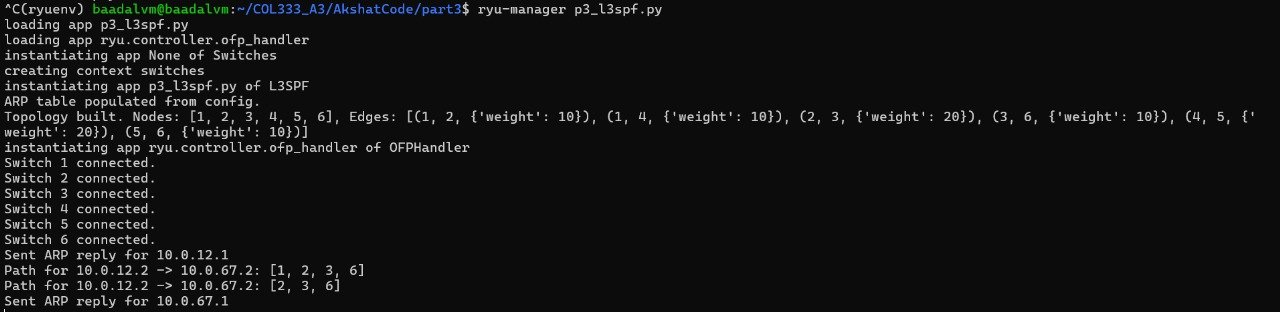
\includegraphics[width=0.9\textwidth]{p3_ping_c.jpeg}
    \caption{Controller logs showing ARP and path calculation for the first ping.}
\end{figure}

\begin{figure}[h!]
    \centering
    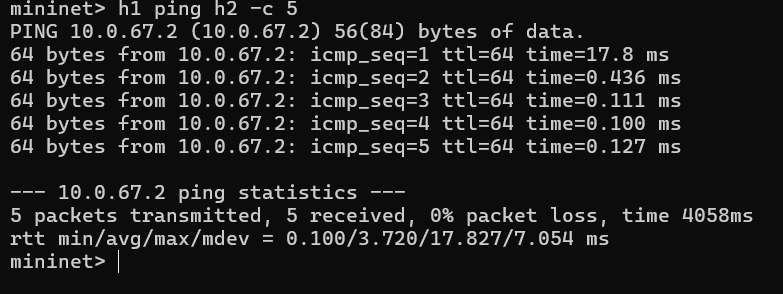
\includegraphics[width=0.9\textwidth]{p3_ping_m.jpeg}
    \caption{Mininet CLI showing results of \texttt{h1 ping h2 -c 5}.}
\end{figure}

\subsubsection*{Observations}
The successful ping with 0\% packet loss confirms that the controller correctly handles inter-subnet routing. The following latency characteristics were observed:
\begin{itemize}
    \item \textbf{Initial Latency:} The first ping has a significantly higher response time (17.8 ms). This is expected behavior as the first packet triggers a table-miss on switch \texttt{s1}, which is sent to the controller. The controller then calculates the shortest path, installs flow rules on all switches along the computed path (\texttt{s1, s2, s4, s6}), and forwards the packet.
    
    \item \textbf{Subsequent Latency:} The next four pings are extremely fast ($<$ 0.5 ms). This is because the necessary flow rules are now installed in the data plane of the switches. These packets are processed directly by the switch hardware at line-rate, bypassing the controller and demonstrating the efficiency of the established forwarding path.
\end{itemize}

\subsection{Installed Flow Rules}
The flow tables of the switches were dumped after the ping test to inspect the installed rules.

\begin{figure}[h!]
    \centering
    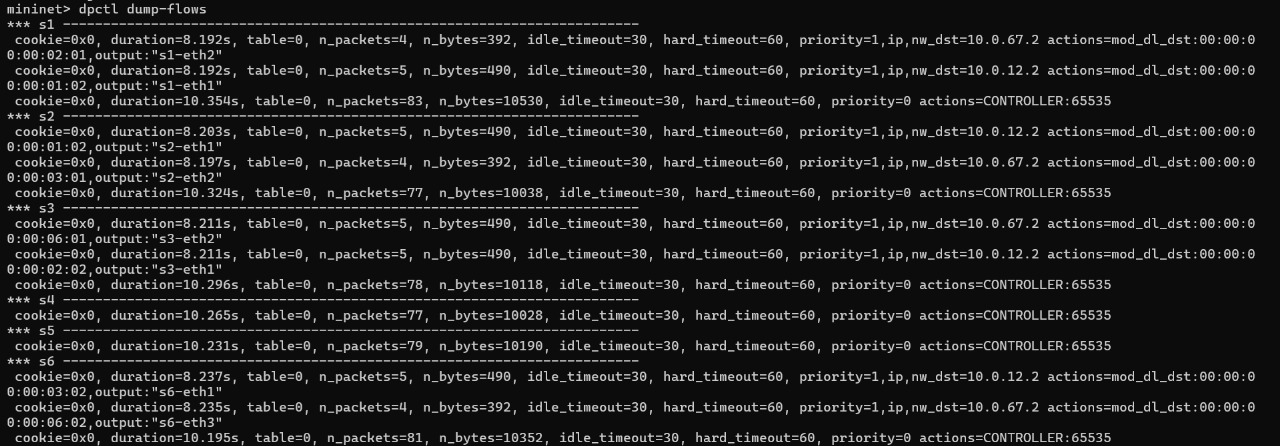
\includegraphics[width=0.9\textwidth]{p3_rules.jpeg}
    \caption{Flow rules installed on switches along the path.}
\end{figure}

\subsubsection*{Observations}
The rules confirm the L3 routing behavior:
\begin{itemize}
    \item Each rule matches on the destination IP address (\texttt{nw\_dst}) only, emulating a traditional routing table.
    \item The actions include \texttt{mod\_dl\_src}, \texttt{mod\_dl\_dst} (MAC address rewriting), and \texttt{DEC\_NW\_TTL} (TTL decrement), which are characteristic of a Layer 3 router.
    \item The final action is \texttt{output:<port>}, forwarding the modified frame to the next hop.
\end{itemize}


\subsection{Assumptions}
The implementation of the L3 routing controller is based on the following key assumptions:
\begin{enumerate}
    \item \textbf{Static Configuration:} The controller relies entirely on the \texttt{p3\_config.json} file for all network information (topology, IPs, MACs). The configuration is assumed to be accurate and complete. No new links can be added on the fly.

    \item \textbf{Centralized ARP Proxy:} The controller intercepts all ARP requests and generates synthetic replies from its static configuration. Hosts do not perform dynamic ARP discovery among themselves.

    \item \textbf{Reactive Path Calculation:} End-to-end paths and their corresponding flow rules are calculated and installed reactively, only upon receiving the first packet of a new flow.

    \item \textbf{Destination-Based Forwarding:} All routing decisions and installed flow rules are based solely on the destination IP address of a packet, consistent with standard IP routing.
\end{enumerate}
\section{Part 4: Comparison with Traditional Routing (OSPF)}

This section details the comparison between a traditional OSPF-based routing setup and our custom SDN controller, focusing on performance during a link failure event.

\subsection{Warm-up Experiment}

Before the failure simulation, a warm-up experiment established a baseline. An \texttt{iperf} test between h1 and h2 confirmed that OSPF had converged and established a stable path, achieving a throughput of approximately 95.5 Mbits/sec (Figure \ref{fig:iperf_warmup}). The established OSPF neighbor relationships (Figure \ref{fig:ospf_neighbors}) and the resulting IP routes on the switches (Figure \ref{fig:ip_route}) confirmed a stable network state prior to the test. Finally, the forwarding rules on switches s1 and s6 were recorded (Figure \ref{fig:ospf_rules}).

\begin{figure}[h!]
    \centering
    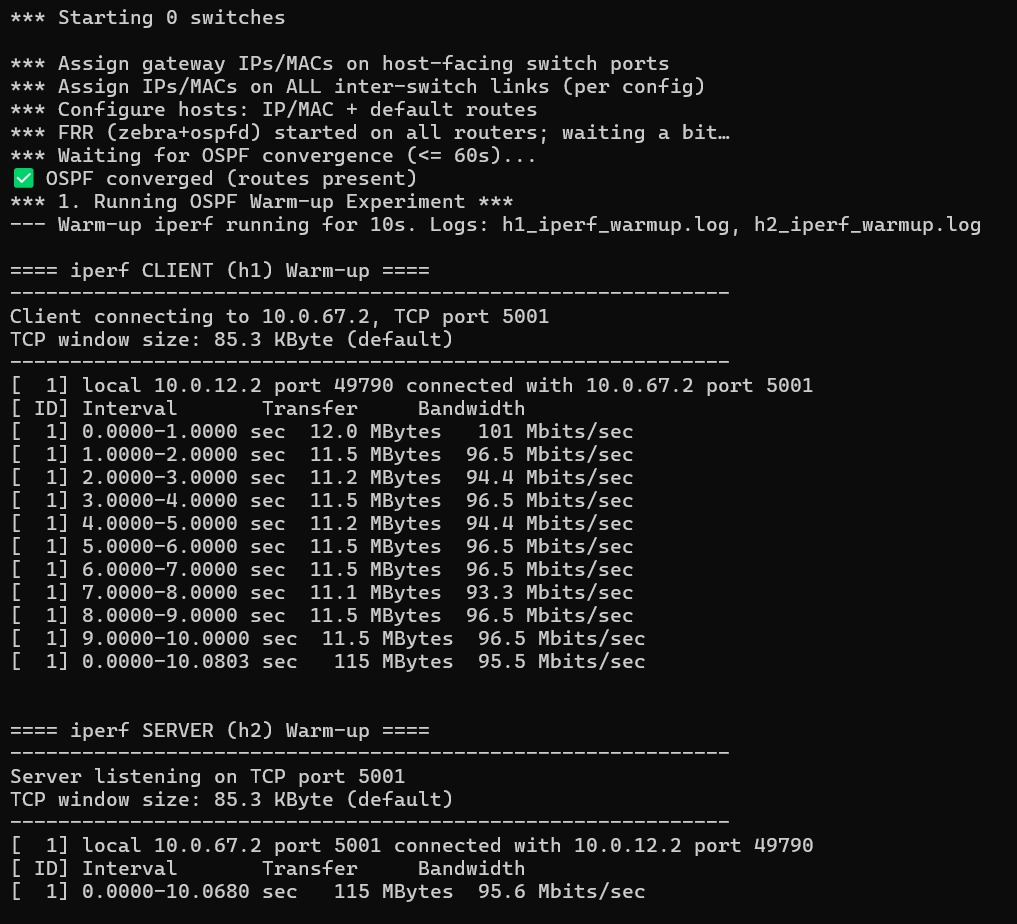
\includegraphics[width=0.9\textwidth]{p4_iperf.jpeg}
    \caption{Baseline \texttt{iperf} throughput between h1 and h2 after OSPF convergence.}
    \label{fig:iperf_warmup}
\end{figure}

\begin{figure}[h!]
    \centering
    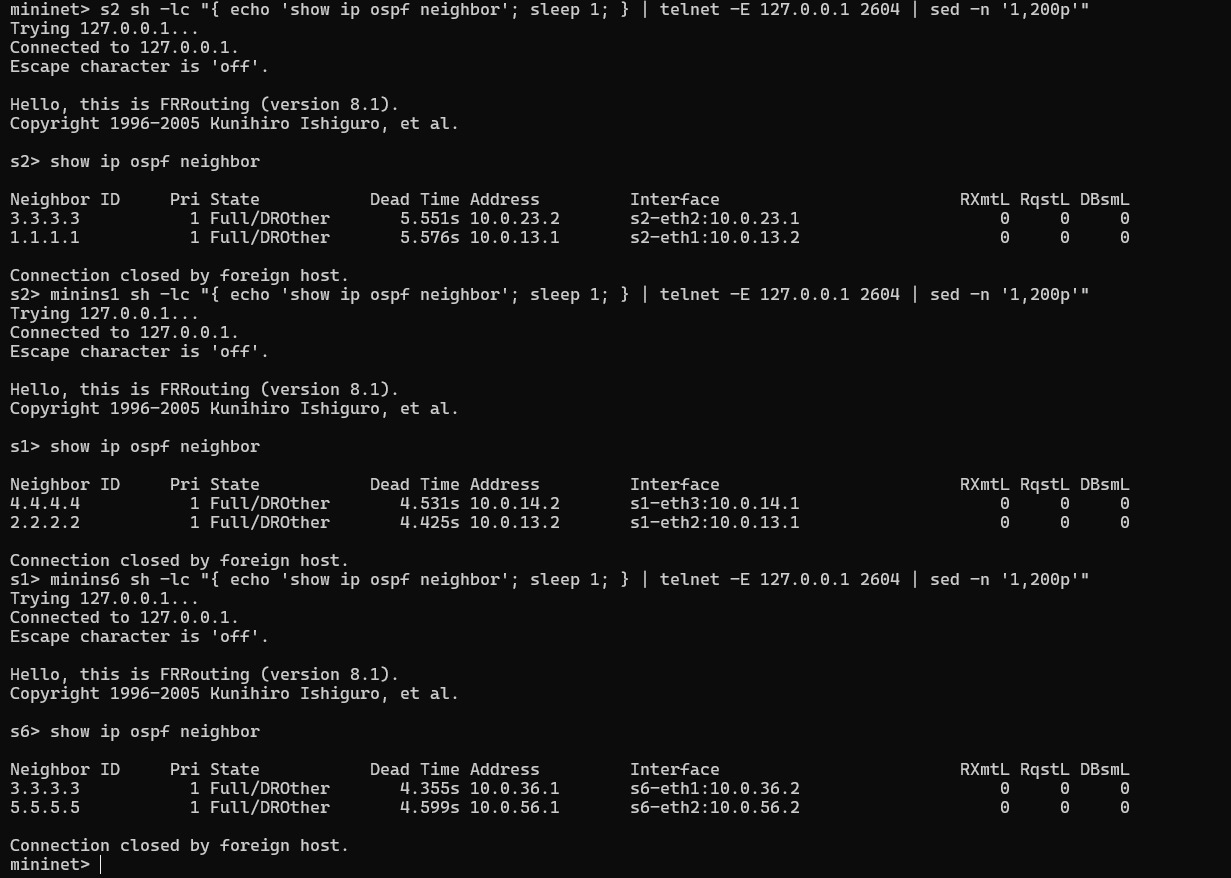
\includegraphics[width=0.9\textwidth]{p4_neighbor.jpeg}
    \caption{OSPF neighbor relationships established on key switches.}
    \label{fig:ospf_neighbors}
\end{figure}

\begin{figure}[h!]
    \centering
    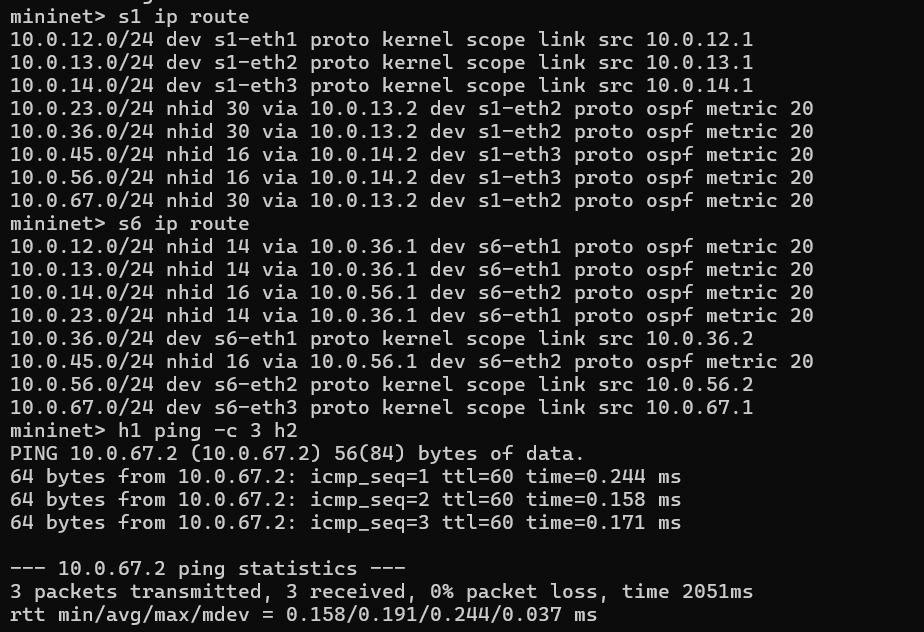
\includegraphics[width=0.9\textwidth]{p4_ip_route_and_ping.jpeg}
    \caption{IP routes and successful ping test after OSPF convergence.}
    \label{fig:ip_route}
\end{figure}

\begin{figure}[h!]
    \centering
    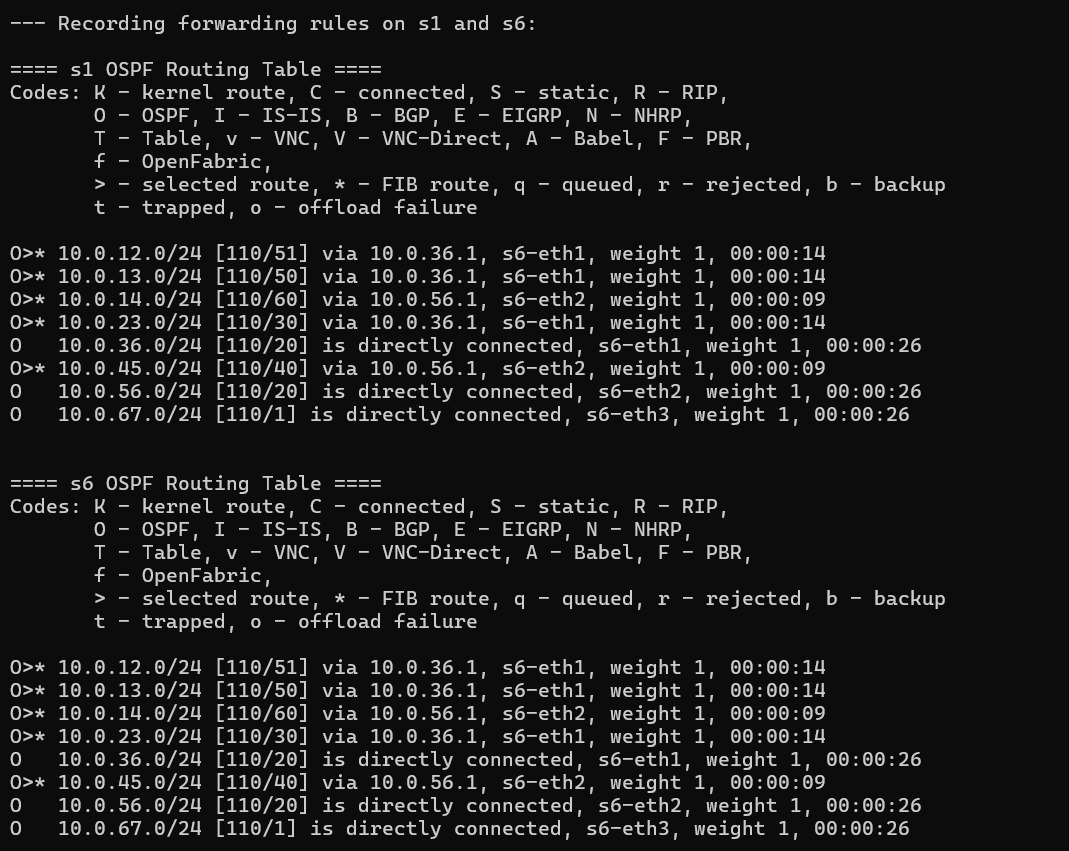
\includegraphics[width=0.9\textwidth]{p4_rules_s1_s6.jpeg}
    \caption{OSPF forwarding rules installed on s1 and s6 after convergence.}
    \label{fig:ospf_rules}
\end{figure}

\subsection{Link Failure Analysis}
The core experiment involved running a 30-second \texttt{iperf} test between h1 and h2, during which a primary link was brought down at T=2s and restored at T=7s. The raw \texttt{iperf} logs provide the data for this analysis.

\subsubsection{OSPF Performance}
\paragraph{Data Plane Convergence}
The plotted throughput graph (Figure \ref{fig:ospf_throughput_graph}) is derived from the client-side \texttt{iperf} logs (Figure \ref{fig:ospf_link_failure_logs}). The data shows the OSPF network reacted to the link failure by rerouting traffic.
\begin{itemize}
    \item \textbf{0-2s:} Throughput is stable at the maximum rate of the primary path ($\approx$100 Mbits/sec).
    \item \textbf{2-3s (Failure):} The link fails. Throughput drops immediately to the alternate path's capacity ($\approx$10 Mbits/sec).
    \item \textbf{7s (Recovery):} The primary link is restored.
    \item \textbf{7-15s:} Throughput remains low on the alternate path while the OSPF control plane re-converges.
    \item \textbf{15s onwards:} Throughput returns to the maximum rate as traffic is redirected back to the primary, faster path.
\end{itemize}
From a data plane perspective, it took OSPF approximately \textbf{8 seconds} (from T=7s to T=15s) to restore traffic to the optimal path after the link was physically restored.

\begin{figure}[h!]
    \centering
    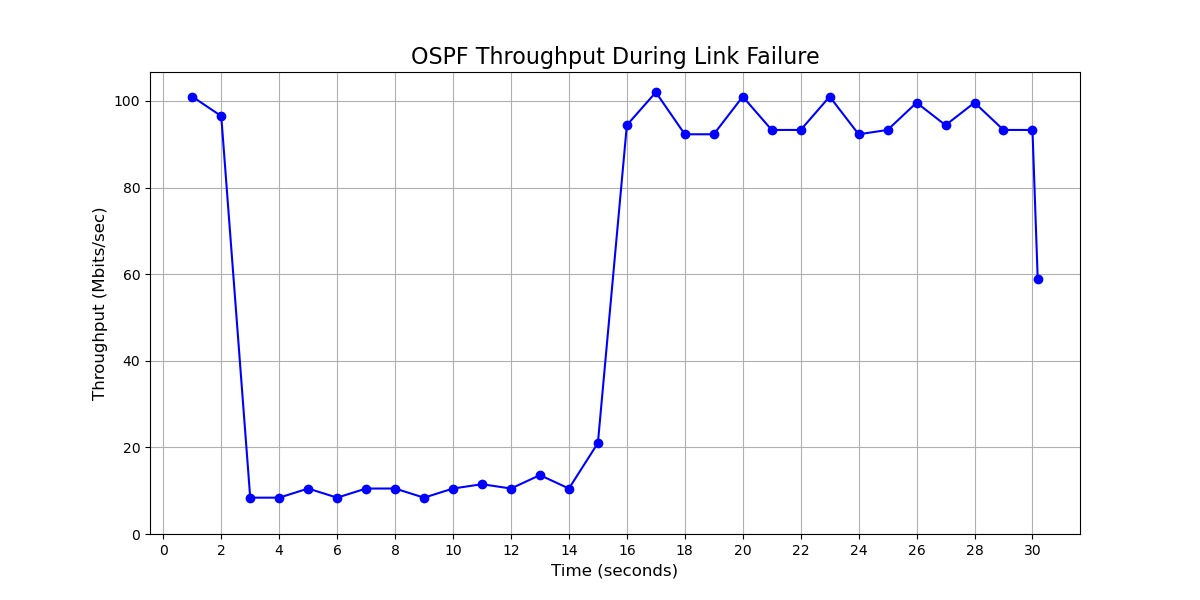
\includegraphics[width=0.9\textwidth]{p4_ospf_thpt_time.jpeg}
    \caption{OSPF throughput graph during the link failure experiment.}
    \label{fig:ospf_throughput_graph}
\end{figure}

\begin{figure}[h!]
    \centering
    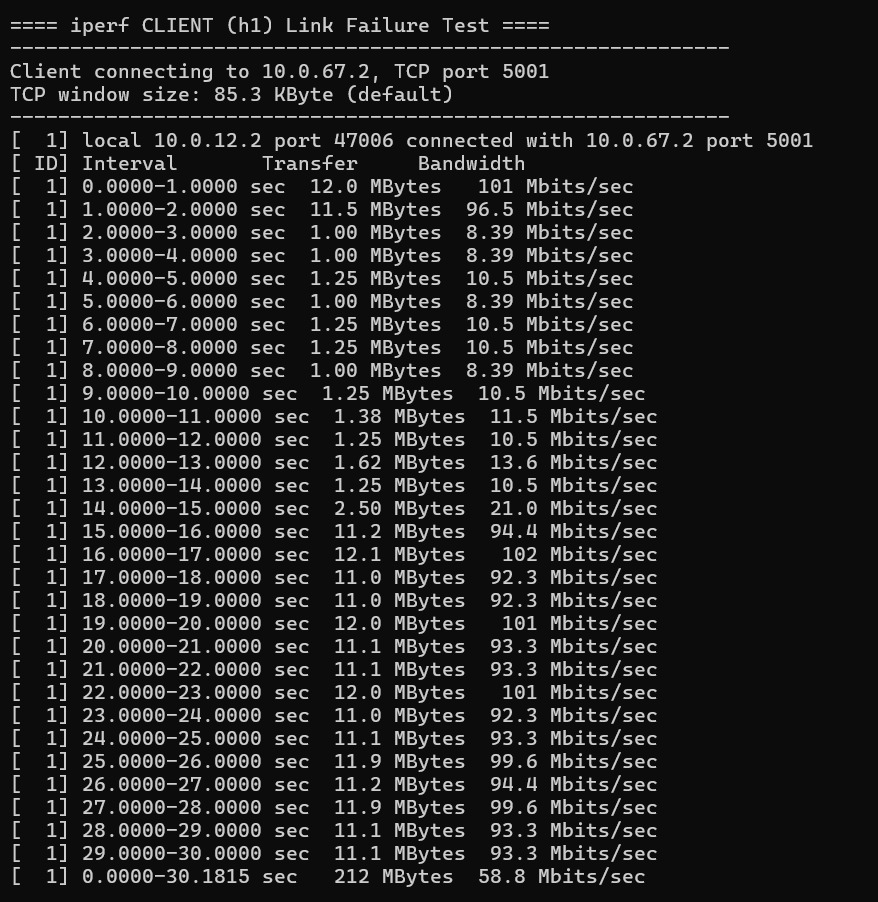
\includegraphics[width=0.9\textwidth]{p4_link_failure_client_ospf.jpeg}
    \caption{Client-side \texttt{iperf} logs for the OSPF link failure test.}
    \label{fig:ospf_link_failure_logs}
\end{figure}

\begin{figure}[h!]
    \centering
    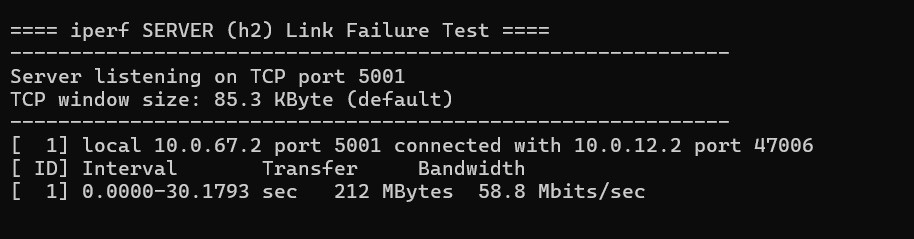
\includegraphics[width=0.8\textwidth]{p4_link_failure_server_ospf.jpeg}
    \caption{Server-side \texttt{iperf} logs for the OSPF link failure test.}
    \label{fig:ospf_link_failure_client_logs}
\end{figure}

\subsubsection{SDN Controller Performance}
\paragraph{Data Plane Convergence}
The SDN controller's recovery profile is plotted in Figure \ref{fig:sdn_throughput_graph}, based on the logs in Figure \ref{fig:sdn_link_failure_logs}.
\begin{itemize}
    \item \textbf{0-2s:} Throughput is stable at the maximum path rate ($\approx$100 Mbits/sec).
    \item \textbf{2s (Failure):} The link fails.
    \item \textbf{2-8s:} Throughput drops to nearly zero, representing a complete data plane outage.
    \item \textbf{7s (Recovery):} The primary link is restored.
    \item \textbf{8-9s:} Throughput rapidly recovers as the controller immediately reinstalls the optimal path.
\end{itemize}
The SDN approach restored traffic to the optimal path within \textbf{2 seconds} of the link's physical recovery.

\begin{figure}[h!]
    \centering
    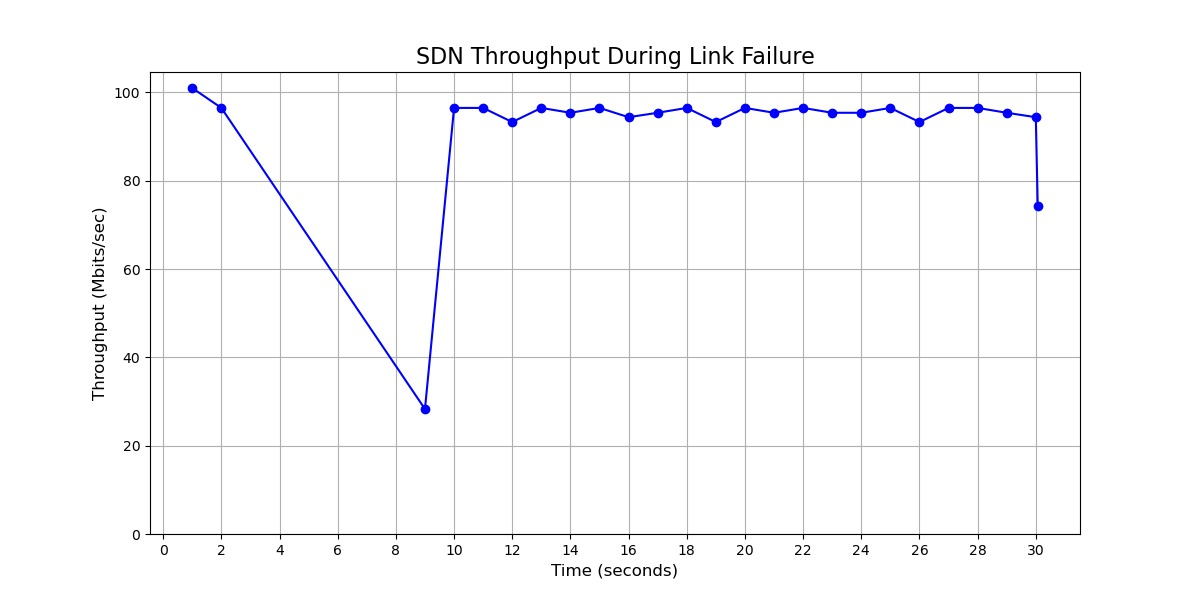
\includegraphics[width=0.9\textwidth]{p4_sdn_thpt_time.jpeg}
    \caption{SDN throughput graph during the link failure experiment.}
    \label{fig:sdn_throughput_graph}
\end{figure}

\begin{figure}[h!]
    \centering
    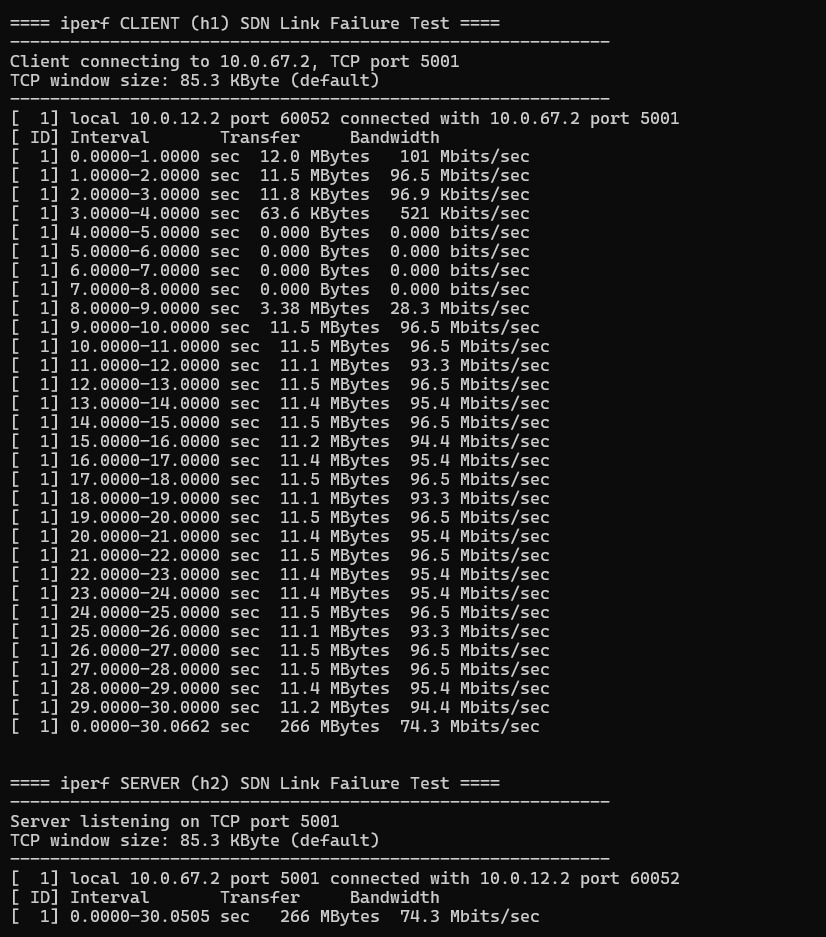
\includegraphics[width=0.9\textwidth]{p4_link_failure_server_sdn.jpeg}
    \caption{Client and server \texttt{iperf} logs for the SDN link failure test.}
    \label{fig:sdn_link_failure_logs}
\end{figure}


\subsection{Comparative Analysis and Conclusion}
The results clearly demonstrate the superior convergence speed of the SDN architecture over traditional, distributed routing protocols like OSPF.

\begin{table}[h!]
\centering
\begin{tabular}{|l|c|c|}
\hline
\textbf{Metric} & \textbf{OSPF} & \textbf{SDN Controller} \\ \hline
\textbf{Control Plane Failure Detection} & $\approx$6 seconds (Timer-based) & Milliseconds (Event-driven) \\ \hline
\textbf{Control Plane Recovery Detection} & $\approx$7 seconds (Adjacency-based) & Milliseconds (Event-driven) \\ \hline
\textbf{Data Plane Recovery to Optimal Path} & $\approx$8 seconds & $\approx$2 seconds \\ \hline
\end{tabular}
\caption{Comparison of OSPF and SDN Convergence Times.}
\label{tab:comparison}
\end{table}

In conclusion, OSPF's convergence is limited by its distributed, timer-based design. In contrast, the SDN controller's centralized global view and event-driven notifications allow it to react almost instantaneously. While this led to a brief, total data plane outage, the network recovered to its optimal state far more quickly than OSPF.
% --------------------------------------------------------------
%     You don't have to mess with anything below this line.
% --------------------------------------------------------------

\end{document}
